\subsection{IU Realizar pago de cita}

\subsubsection{Objetivo}
Registrar el pago de una cita para que el paciente pueda acceder a ésta.

\subsubsection{Diseño}
Esta pantalla aparece al hacer click sobre \IUbutton{Realizar pago de cita} al haber iniciado sesión como cajero.

\begin{figure}[htbp!]
	\centering
	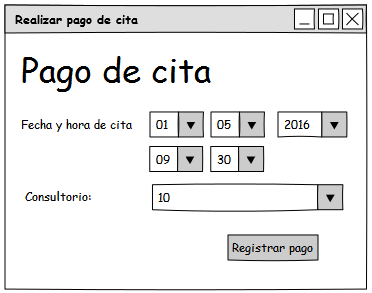
\includegraphics[width=0.8\textwidth]{images/IU_pagar_cita}
	\caption{IU Realizar pago de cita}
\end{figure}


\subsubsection{Salidas}
\begin{itemize} 
	\item Mensaje de confirmación: Cadena ``Pago registrado correctamente"
	\item Información de cita:
	\begin{itemize}
		\item Fecha de cita: Fecha en formato dd/mm/yyyy
		\item Hora de cita: Hora con formato hh:mm
		\item Consultorio de cita: Número entero entre 1 y 12
	\end{itemize}
\end{itemize}
\subsubsection{Entradas}
\begin{itemize}
	\item Fecha de la cita: Fecha en fomato dd/mm/yyyy [Requerido]
	\item Hora de cita: hora en formato hh:mm [Requerido]
	\item Número de consultorio: Número positivo entre 0 y 12 [Requerido]
\end{itemize} 

\subsubsection{Comandos}
\begin{itemize}
	\item \IUbutton{Registrar pago}:  Verifica que el la cita exista, tenga fecha y hora posterior a las actuales y haya sido pagada. En tal caso, se actualiza el estado de la cita a pagada.  \IUref{UI2}{Home}.	
\end{itemize}

\subsubsection{Mensajes}
\begin{Citemize}
	\item {\bf MSGb} Cita no existe
	\item {\bf MSGc} La cita expiró
	\item {\bf MSGd} Cita ya está pagada
	\item {\bf MSGe} Complete todos los campos
	\item {\bf MSGf} Formato de campos inválido
\end{Citemize}

\subsection{IU Crear expediente}

\subsubsection{Objetivo}
Registrar los datos y antecedentes médicos de un paciente.

\subsubsection{Diseño}
Esta pantalla aparece al hacer click sobre \IUbutton{Atender paciente} y es la primera consulta del paciente, al haber iniciado sesión como médico.

\begin{figure}[htbp!]
	\centering
	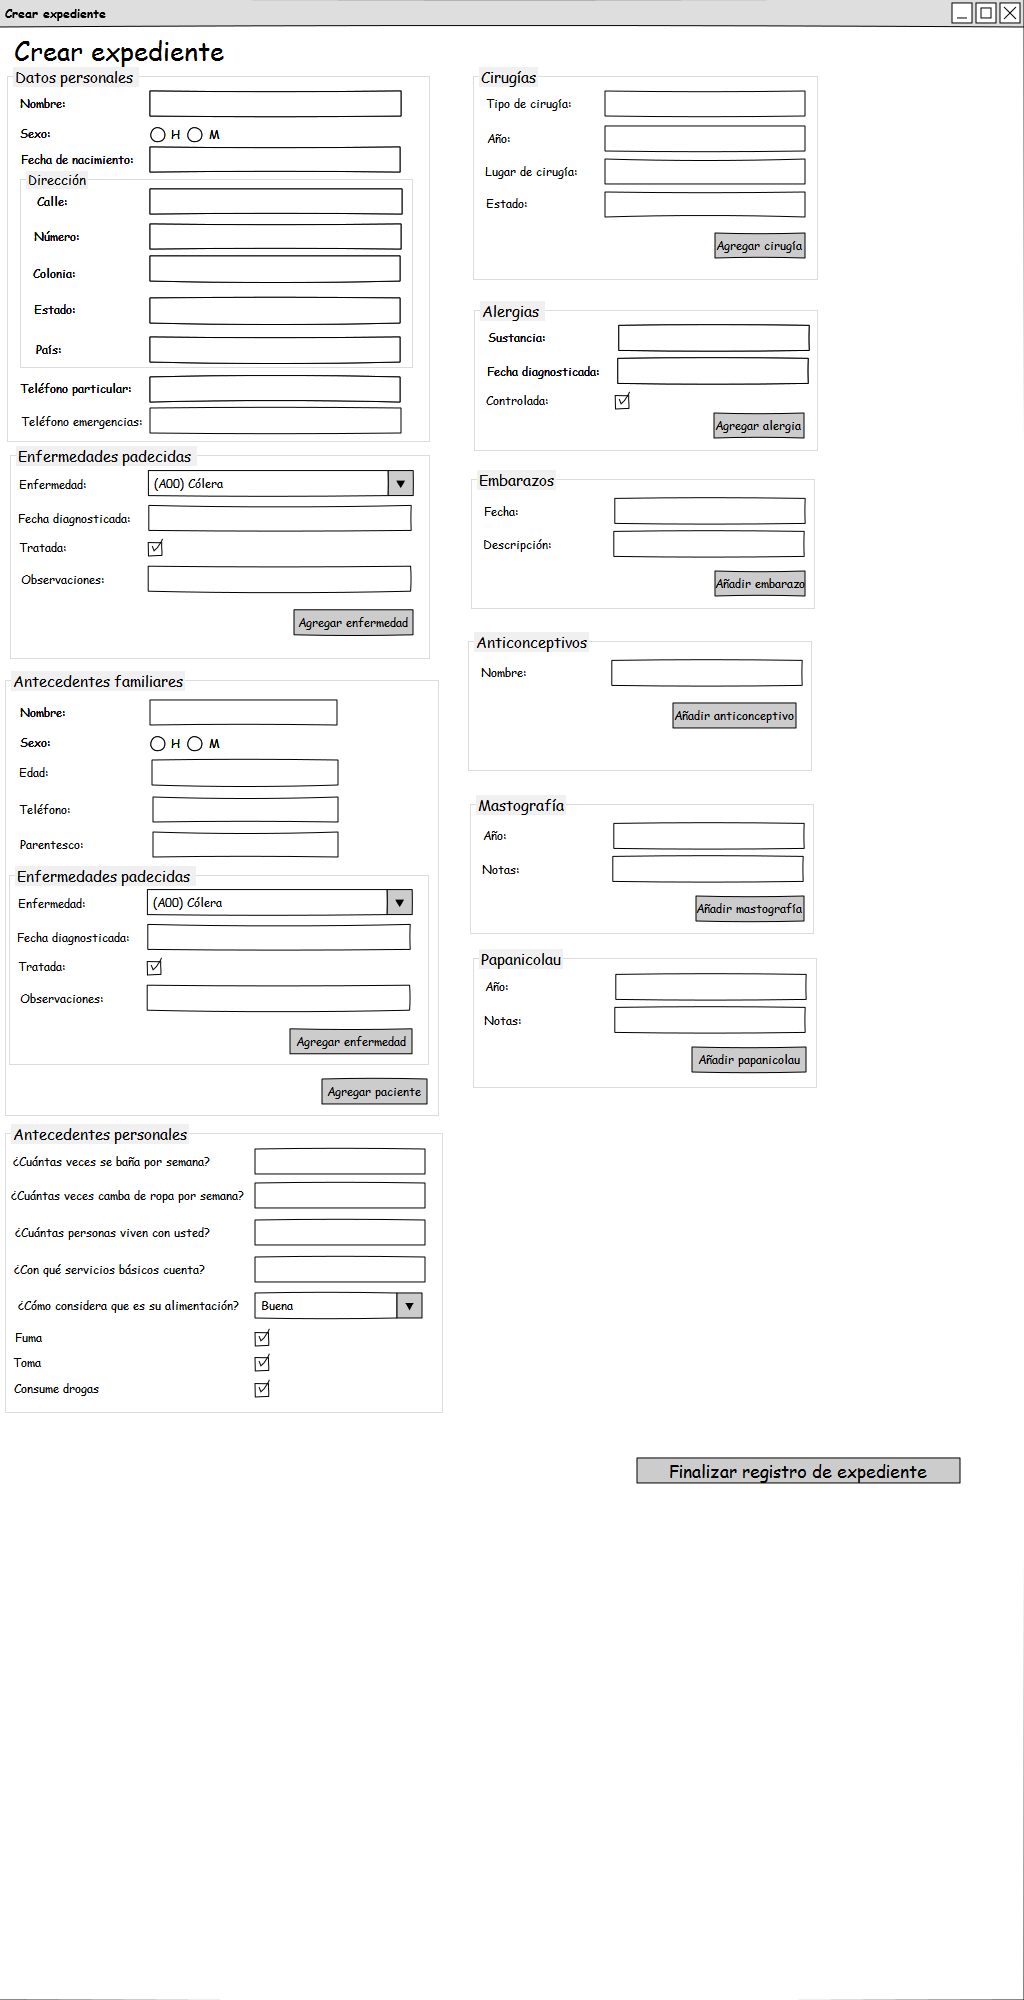
\includegraphics[width=0.8\textwidth]{images/IU_crear_expediente}
	\caption{IU Crear expediente}
\end{figure}


\subsubsection{Salidas}
\begin{itemize} 
	\item Listadas en el caso de uso CU6 ``Crear expediente"
\end{itemize}
\subsubsection{Entradas}
\begin{itemize}
	\item Listadas en el caso de uso CU6 ``Crear expediente"
\end{itemize}

\subsubsection{Comandos}
\begin{itemize}
	\item \IUbutton{Finalizar registro de expediente}:  Verifica que hayan sido ingresados los datos requeridos y tengan formato correcto, de ser así, se guardan datos del expediente y se notifica al médico.  \IUref{UI2}{Home}.	
	\item \IUbutton{Agregar enfermedad}:  Agrega un elemento a la lista de enfermedades del paciente o de un familiar .
	\item \IUbutton{Agregar familiar}:  Agrega un elemento a la lista de antecedentes familiares del paciente .
	\item \IUbutton{Agregar cirugía}:  Agrega un elemento a la lista de cirugías del paciente .
	\item \IUbutton{Agregar alergia}:  Agrega un elemento a la lista de alergias del paciente .
	\item \IUbutton{Agregar embarazo}:  Agrega un elemento a la lista de embarazos del paciente .
	\item \IUbutton{Agregar anticonceptivo}:  Agrega un elemento a la lista de anticonceptivos del paciente .
	\item \IUbutton{Agregar mastografía}:  Agrega un elemento a la lista de mastografías del paciente .
	\item \IUbutton{Agregar papanicolau}:  Agrega un elemento a la lista de papanicolaus del paciente .
\end{itemize}

\subsubsection{Mensajes}
\begin{Citemize}
	\item {\bf MSGa} Expediente creado correctamente
	\item {\bf MSGb} Complete todos los campos
	\item {\bf MSGc} Formato de campos inválido
\end{Citemize}


\subsection{IU registrar médico}

\subsubsection{Objetivo}
Registrar un médico para que pueda atender citas.

\subsubsection{Diseño}
Esta pantalla aparece al hacer click sobre \IUbutton{Registrar médico} al haber iniciado sesión como gerente.

\begin{figure}[htbp!]
	\centering
	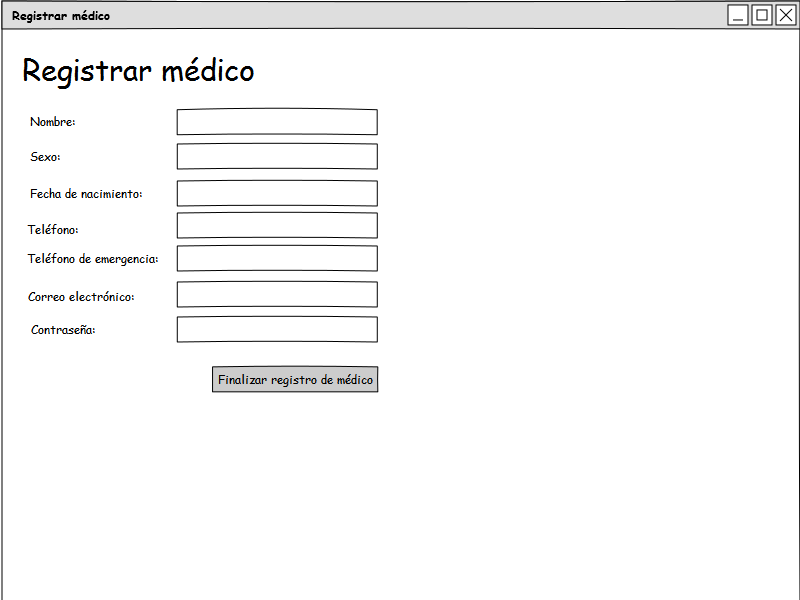
\includegraphics[width=0.8\textwidth]{images/IU_registrar_medico}
	\caption{IU Registrar médico}
\end{figure}


\subsubsection{Salidas}
\begin{itemize} 
	\item Mensaje de confirmación: Cadena ``Médico registrado correctamente"
\end{itemize}
\subsubsection{Entradas}
\begin{itemize}
	\item Email del médico: cadena de texto compuesta de 4 partes [requerido]:  
	\begin{itemize}
		\item cadena de texto.
		\item carácter ‘@’
		\item cadena que identifica al servidor que brinda el servicio de correo electrónico
		\item carácter ‘.’ y dominio
	\end{itemize}
	\item *Contraseña:  Cadena de longitud mínima de 8 caracteres
	\item Lista de datos personales [todos requeridos]
	\begin{itemize}
		\item Nombre: Constituido por nombre(s) y apellidos.Cádena de caracteres
		\item Sexo  Caracter 'H' o 'M' (hombre,mujer)
		\item Fecha de nacimiento: Formato de fecha DD/MM/AAAA
		\item Teléfono: Cadena de 8 a 20 dígitos
		\item Teléfono de emergencia: Cadena de 8 a 20 dígitos
		
	\end{itemize}
\end{itemize}

\subsubsection{Comandos}
\begin{itemize}
	\item \IUbutton{Finalizar registro de médico}:  Verifica que los datos requeridos hayan sido ingresados, que los datos ingresados tengan un formato correcto y que no exista un médico registrado con el mismo correo elctrónico. En tal caso se guarda la información del médico.  \IUref{UI2}{Home}.	
\end{itemize}

\subsubsection{Mensajes}
\begin{Citemize}
	\item {\bf MSGa} El correo electrónico proporcionado ya está registrado
	\item {\bf MSGb} Complete todos los campos
	\item {\bf MSGc} Formato de campos inválido
\end{Citemize}


\subsection{IU registrarse paciente}

\subsubsection{Objetivo}
Que un paciente se registre para poder agendar citas.

\subsubsection{Diseño}
Esta pantalla aparece al hacer click sobre \IUbutton{Registrarse como paciente}.

\begin{figure}[htbp!]
	\centering
	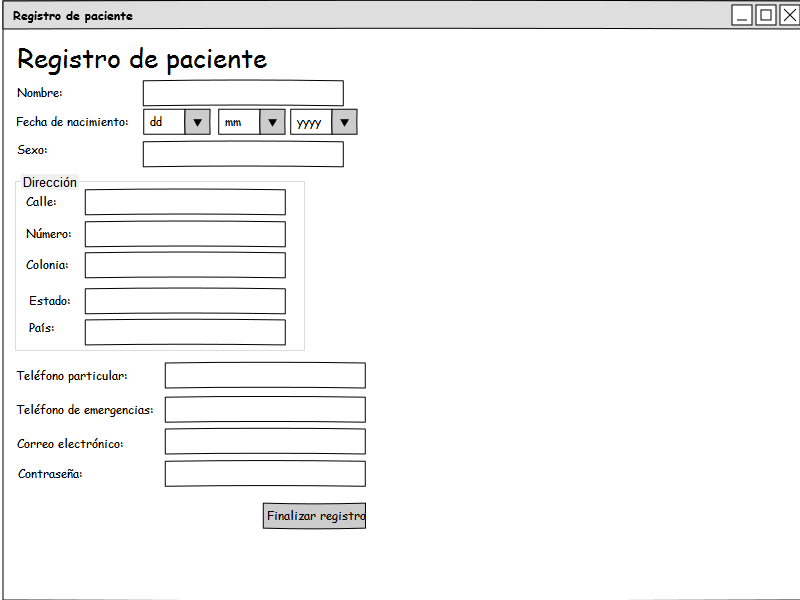
\includegraphics[width=0.8\textwidth]{images/IU_registrarse_paciente}
	\caption{IU Registrarse paciente}
\end{figure}


\subsubsection{Salidas}
\begin{itemize} 
	\item Mensaje de confirmación: Cadena ``Paciente registrado correctamente"
\end{itemize}
\subsubsection{Entradas}
\begin{itemize}
	\item *Email del paciente: cadena de texto compuesta de 4 partes:  
	\begin{itemize}
		\item cadena de texto.
		\item carácter ‘@’
		\item cadena que identifica al servidor que brinda el servicio de correo electrónico
		\item carácter ‘.’ y dominio
	\end{itemize}
	\item* Nombre completo del paciente:  3 cadenas de caracteres (Nombre(s), apellido paterno, apellido materno).
	\item *Fecha de nacimiento del paciente: Fecha DD/MM/AAAA
	\item *Sexo del paciente: 1 carácter . ‘H’ para hombre, ‘M’ para mujer.
	\item Dirección
	\begin{itemize}
		\item *Calle: Cádena de caracteres.
		\item Número: Cádena de caracteres.
		\item *Colonia: Cádena de caracteres.
		\item *Estado: Cádena de caracteres.
		\item *País : Cádena de caracteres.
		\item Teléfono particular: Cádena de 8 a 10 caracteres.
		\item Teléfono de emergencia: Cádena de 8 a 10 caracteres.
	\end{itemize}    
	\item *Contraseña:  Cadena de longitud mínima de 8 caracteres
\end{itemize}

\subsubsection{Comandos}
\begin{itemize}
	\item \IUbutton{Finalizar registro de paciente}:  Verifica que los datos requeridos hayan sido ingresados, que los datos ingresados tengan un formato correcto y que no exista un paciente registrado con el mismo correo elctrónico. En tal caso se guarda la información del paciente.  \IUref{UI2}{Home}.	
\end{itemize}

\subsubsection{Mensajes}
\begin{Citemize}
	\item {\bf MSGa} El correo electrónico proporcionado ya está registrado
	\item {\bf MSGb} Complete todos los campos
	\item {\bf MSGc} Formato de campos inválido
\end{Citemize}